\subsection{Servo}
On the vehicle there is a servo, which is a S3003 by Futaba.
The servo is used for the steering of the vehicle. The servo controls the steering through breaking one of the belts and transfer that power over to the other belt, thanks to the differential gear box.


The Servo is controlled by a PWM signal. The received PWM signal is converted into an angle by the servo to control the steering of the belts, as seen on \figref{timeVSangle}. An angle of 90° is the normal position for going straight, while 0° and 180° are the limits for turning, where one of the belts is not moving. 

A mechanical arm is mounted on the servo and connected to the brakes of the tracks. When the servo rotates one way, it triggers the brakes more on one side and less on the other side, according to the value of the angle sent, through the PWM signal. This way, one of the belt will drive slower and the other belt drive faster, which will make the vehicle turn, without decreasing the motor power.

The servo reacts linearly to the PWM signal and the cycle of the signal is 30 milliseconds. To get the servo to be in neutral position, the servo needs a PWM signal of 4.83 \% (a period of 1450 microseconds). For 180°, it is 8.33 \% (a period of 2500 microseconds) and 1.67 \% (a period of 500 microseconds) for 0°. \\

%source http://www.societyofrobots.com/actuators_servos.shtml\\

\begin{figure}[H]
	\centering
	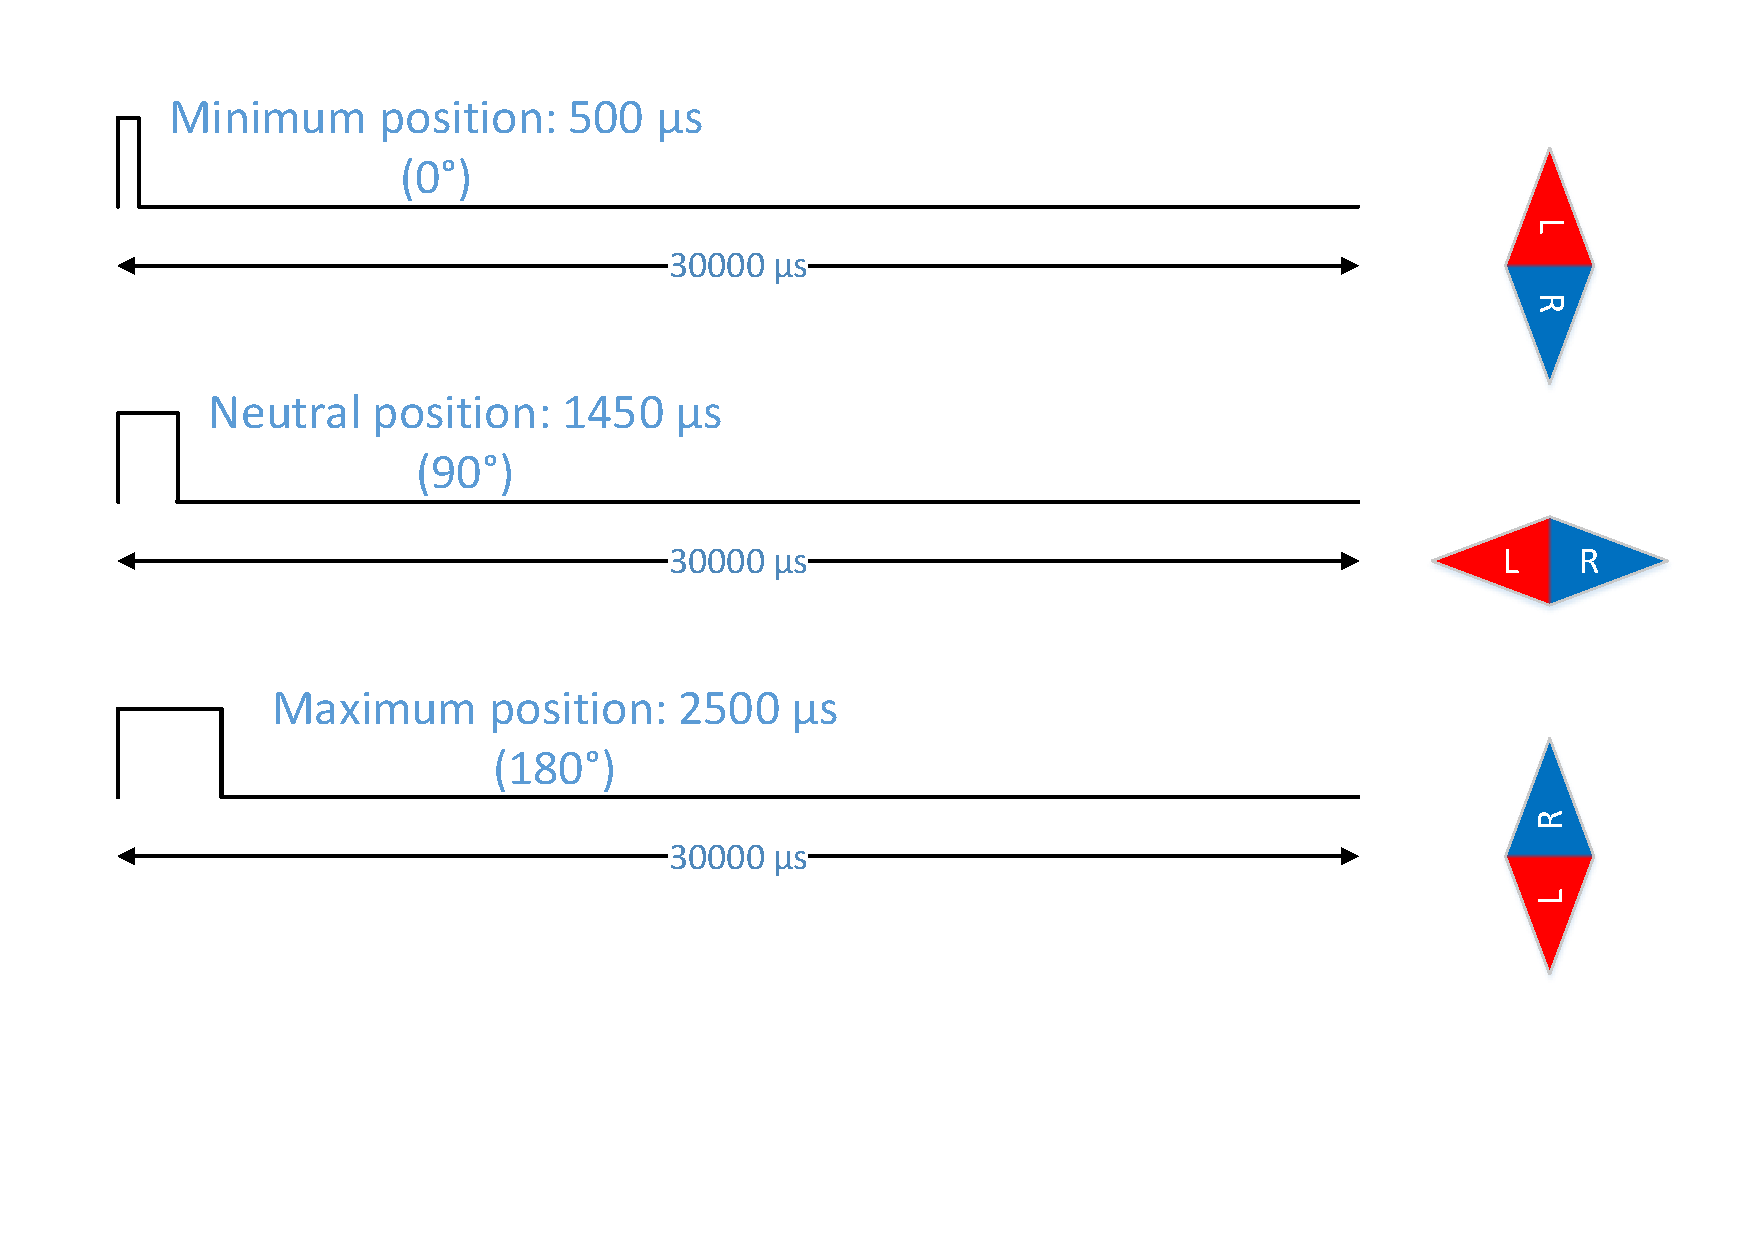
\includegraphics[scale=0.6]{figures/TimeVSangle.pdf}
	\caption{Convertion from time to angle by the servo}
	\label{timeVSangle}
\end{figure}

